%%%%%%%%%%%%%%%%%%%%%%% file moduleX_template.tex %%%%%%%%%%%%%%%%%
%
%
% This is a template for creating your papers for the course KRW
% It is based on the standard Latex template for Springer publications
% but contains a suggestion for the structure and some content of the 
% paper. 
%
% Please adapt this document wherever needed.
%
% For more information about the required Latex Style check the document
% typeinst.pdf in the StyleFiles directory. 
%
%%%%%%%%%%%%%%%%%%%%%%%%%%%%%%%%%%%%%%%%%%%%%%%%%%%%%%%%%%%%%%%%%%%%%%%%%


\documentclass[runningheads,a4paper]{../../StyleFiles/llncs}

\usepackage{url}
\usepackage{graphicx}
\usepackage{amssymb}
\usepackage{listings}
\lstset{language=SQL,morekeywords={PREFIX,java,rdf,rdfs,url}}
 

\newcommand{\keywords}[1]{\par\addvspace\baselineskip
\noindent\keywordname\enspace\ignorespaces#1}

\begin{document}

\mainmatter  % start of an individual contribution

% first the title is needed
\title{Data- and Systems Paper : Finding Amsterdam}

% a short form should be given in case it is too long for the running head
\titlerunning{Data- and Systems Paper}

% the name(s) of the author(s) follow(s) next
%
% NB: Chinese authors should write their first names(s) in front of
% their surnames. This ensures that the names appear correctly in
% the running heads and the author index.
%
\author{Alivanistos, Dimitris. \\ Baez, Selene. \\ Jemmett, Andrea. }
%
\authorrunning{Alivanistos, Dimitris. \\ Baez, Selene. \\ Jemmett, Andrea.}
% (feature abused for this document to repeat the title also on left hand pages)

% the affiliations are given next; don't give your e-mail address
% unless you accept that it will be published
\institute{\url{d.alivanistos@student.vu.nl} \and \url{s.baezsantamaria@student.vu.nl} \and \url{a.jemmett@student.vu.nl}}

\maketitle


\begin{abstract}
The abstract should summarize the contents of the paper and should
contain at least 70 and at most 150 words. It should be written using the
\emph{abstract} environment.
\end{abstract}


\section{Introduction}
In the journey of having a Semantic Web where everything is linked, open and reusable, dealing with volume is necessary. The same way as in "Finding Wally", the tangled world of Linked Data makes it virtually impossible to find some specific information. The problem becomes even more complex when the information to be retrieved is not clear, in which case the task is comparable to fishing in the darkness.

Given the trends in the Semantic Web, it is undeniable that finding specific information, and reasoning in large heterogeneous datasets will become a need. Thus efficient mechanisms are required to achieve these goals. In fact, this year's \textit{International Semantic Web Conference} \footnote{\url{http://iswc2016.semanticweb.org/pages/calls/research-track.html}}, held in Kobe, Japan, recognizes it as one of the main topics of interest, phrasing it as "Architectures and algorithms for extreme volume, heterogeneity, dynamicity, and decentralization of Semantic Web data"

In this paper we address the previous challenge with approximation techniques as a tool for efficient reasoning over a large dataset. To link this to our previous work, we select the specific domain of Geographical Locations, and aim to retrieve all the information related to The Netherlands from the provided \texttt{dataset} in Stardog.  

The goal of this assignment is to perform approximation techniques by a smart selection of nodes that successfully retrieve all, or nearly all, information related to The Netherlands. 

\section{Related Work}
Regardless of its importance, very few research has been done to deal with volume on the Semantic Web. So far, the growth rate of the Web is winning the race against scientist trying to analyse it accurately within reasonable time. As mentioned by many researchers in the field of the Semantic Web, reasoning with large or complex terminology is one of the well-known bottlenecks in application of ontologies, because of the computational difficulty of the task.

As early as 2007, Schlobach et al. \cite{schlobach2007anytime} proposed approximation techniques based on logical assumptions of monotonicity. These techniques aimed to reduce the volume of data in order to improve on the running time, without loosing any or most of the logic entailment. Similar to us, they compared the selection of random axioms to two more sophisticated methods of selection. However, their procedure is based on frequency, either taking the most or least occurring entities, while we propose a degree approach, taking the best well-connected entities.

Another perspective was introduced by Mika and Tummarello \cite{mika2008web} who proposed to use Grid Computing to tackle the problem of volume. As stated in their paper, parallelism can be used in order to analyse, query and reason with large scale RDF Data. Specifically for complex reasoning tasks, the strategy described includes the use of several “reasoning servers” shared across MapReduce jobs, which then cache reasoning results in large main memories, in order to complete the task at hand.

\section{The dataset}
\textit{Laundromat}\footnote{\url{http://lodlaundromat.org/}} is a tool for cleaning data that provides well-formed datasets of different domains and volumes \cite{beek2014lod}. Searching the LOD for sets linked to the OWL ontology, one can find a set of ontologies that are expressive and complex enough to pose a challenge in the context of this assignment. Merging of some of the previous produced the \texttt{dataset} that we work on in this milestone. This \texttt{datset} was provided to us via the StarDog server. 

At a first glance, the \texttt{dataset} is particularly challenging because of many varied reasons, mainly:

\begin{enumerate}
	\item \textbf{Volume}: The given dataset is about 200 times larger than the ontology we created for the previous milestones.
	\item \textbf{Heterogeneity}: It is composed by several ontologies from different domains (e.g the foaf \footnote{Friend of a friend ontology \url{http://lov.okfn.org/dataset/lov/vocabs/foaf}}, a wine ontology, a scientific-research ontology and a tourism ontology). Furthermore it comprises several different languages.
	\item \textbf{Decentralization}: There is no central ontology that acts as an intermediate node for other ontologies to connect.
\end{enumerate}

Due to the above attributes, unforeseen challenges need to be tackled. These were not present in the well-designed dataset that we created previously, therefore the reasoning methods we used before are not sufficient and need to be extended.

\section{Data Analytics}
Before reasoning or extracting any valuable information about the \texttt{dataset}, we first need to delve deeper into it to understand its content. In order to get more details, we perform an exploratory study of its most basic statistical characteristics. We do this in a 3-step process that we describe in the following subsections.

\subsection{Step 1: Query for finding the different ontologies}
First we need to characterize the content of the \texttt{dataset} by the domains it refers to. To do so we query the \texttt{dataset}, using Stardog as endpoint, to get the ontologies that are present. The query is presented in Listing \ref{ontology_query}.

\begin{lstlisting}[captionpos=b, caption=SPARQL query for getting different Ontologies in the \texttt{dataset}, label=lst:sparql, basicstyle=\ttfamily\small,frame=bt]
SELECT DISTINCT ?entity ?elabel ?type ?tlabel 
WHERE { 
	?entity a ?type .
	?type rdfs:label 'Ontology' .
	OPTIONAL { ?entity rdfs:label ?elabel } . 
	OPTIONAL { ?type rdfs:label ?tlabel } 
}
\end{lstlisting}
\label{ontology_query}

We note that the \texttt{dataset} is composed of 103 ontologies with seemingly unrelated domains. Some examples are listed here:

\begin{itemize}
	\item \url{http://www.kanzaki.com/ns/music}: A music vocabulary
	\item \url{http://www.w3.org/TR/2003/PR-owl-guide-20031209/wine}: A wine ontology
	\item \url{http://aims.fao.org/aos/geopolitical.owl}: A geopolitical ontology
	\item \url{ http://rhizomik.net/ontologies/copyrightonto.owl}: A copyright ontology
\end{itemize}

\subsection{Step 2: Frequency of classes}
Secondly, we would like to count the class occurrences in the \texttt{dataset}, similar to Schlobach et al \cite{schlobach2007anytime}. To do so, we obtain frequency statistics using the following query:

\begin{lstlisting}[captionpos=b, caption=SPARQL query for getting class frequencies, label=lst:sparql, basicstyle=\ttfamily\small,frame=bt]
SELECT ?class (COUNT(?resource) as ?count) 
WHERE {
	?resource a ?class . 
} GROUP BY ?class ORDER BY DESC(?count)
\end{lstlisting}

The most frequent class is owl:Thing with 138,568 occurrences. Interestingly the second most frequent class is not the owl:Class, with 36,273 occurrences, but a class related to provenance as opmo:WasControlledBy with 38,165 occurrences. More details on the top 10 classes is given in Table \ref{frequency_table}. A visualization of the frequencies is shown in Figure \ref{fig:frequency}, excluding the first (owl:Thing) due to axis boundaries.

\begin{table}[h]
	\begin{center}
		\begin{tabular}{| l | c |}
			\hline
			\textbf{Class} & \textbf{Count} \\ \hline
			owl:Thing &	138568 \\ \hline
			http://openprovenance.org/model/opmo\#WasControlledBy & 38165 \\ \hline
			owl:Class &	36273 \\ \hline
			owl:Restriction	& 30554 \\ \hline
			http://vivoweb.org/ontology/core\#DateTimeValue &	27041 \\ \hline
			http://vivoweb.org/ontology/core\#DateTimeInterval &	24804 \\ \hline
			http://vivoweb.org/ontology/core\#Role &	23561 \\ \hline
			http://vivoweb.org/ontology/core\#TeacherRole &	23373 \\ \hline
			http://vivoweb.org/ontology/core\#Relationship &	20946 \\ \hline
			http://vivoweb.org/ontology/core\#Authorship &	20938 \\ \hline
		\end{tabular}
		\caption{Top 10 classes with respect to frequency in \texttt{dataset}.}
		\label{frequency_table}
	\end{center}
\end{table}

\begin{figure}[h]
	\centering
	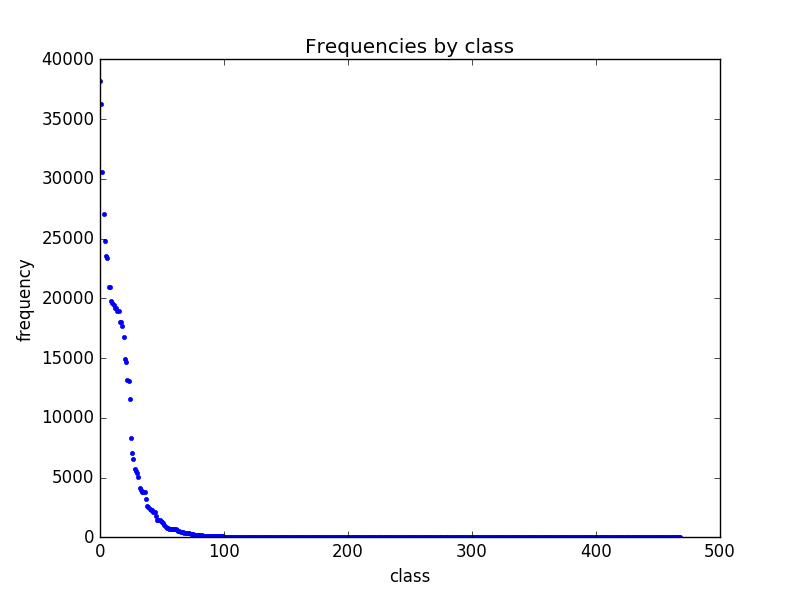
\includegraphics[width=.7\textwidth]{img/dataset_frequency.png}
	\caption{Plot of frequencies for classes in \texttt{dataset}. \textit{owl:Thing} is excluded.}
	\label{fig:frequency}
\end{figure}

\subsection{Step 3: Degree}
Finally, inspired by network analytics we decided to calculate the in-degree and out-degree of each entity. This time the queries could not be computed directly in the Stardog web application, since it automatically handles the limits of the queries and truncates the results. Therefore, we create our own Python script to submit queries to the Stardog endpoint and get full results. 

The in-degree and out-degree queries are shown in the following two Listings:

\begin{lstlisting}[captionpos=b, caption=SPARQL query for calculating in degree of entities, label=lst:sparql, basicstyle=\ttfamily\small,frame=bt]
SELECT DISTINCT ?entity
	(COUNT(distinct ?pin) as ?indegree)
	WHERE { 
		?entity a owl:Thing .
		?something ?pin ?entity .
	}
GROUP by ?entity
ORDER by desc(?indegree)
\end{lstlisting}

\begin{lstlisting}[captionpos=b, caption=SPARQL query for calculating out degree of entities, label=lst:sparql, basicstyle=\ttfamily\small,frame=bt]
SELECT DISTINCT ?entity
	(COUNT(distinct ?pout) as ?outdegree)
	WHERE { 
		?entity a owl:Thing .
		?entity ?pout ?somethingelse .
	}
GROUP by ?entity
ORDER by desc(?outdegree)
\end{lstlisting}

We observe an increase in the time complexity for these queries. The in-degree query takes 55 seconds, while out-degree query takes 46 seconds, compared to the queries in the previous two subsections that are performed almost instantaneously. 

The results for in-degree range between [1, 13] while the ones for out-degree lie in the range of [1, 81]. Figures \ref{fig:indegree} and \ref{fig:outdegree} visualize the distributions.

\begin{figure}[h]
	\centering
	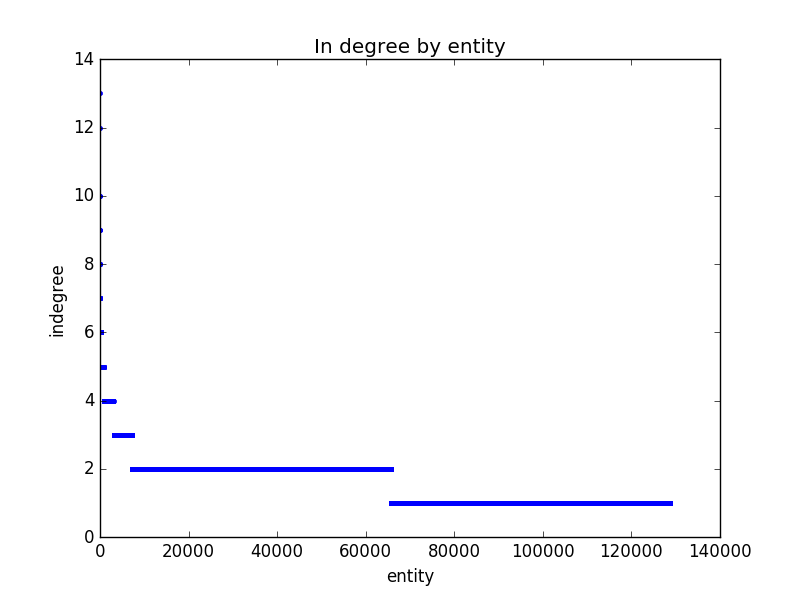
\includegraphics[width=.7\textwidth]{img/dataset_indegree.png}
	\caption{Plot of in-degree for entities in \texttt{dataset}.}
	\label{fig:indegree}
\end{figure}

\begin{figure}[h]
	\centering
	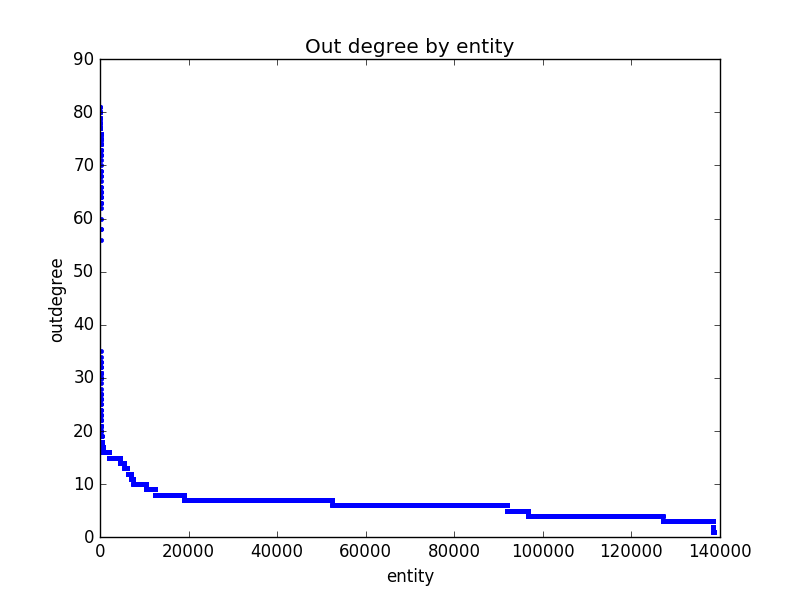
\includegraphics[width=.7\textwidth]{img/dataset_outdegree.png}
	\caption{Plot of out-degree for entities in \texttt{dataset}.}
	\label{fig:outdegree}
\end{figure}

\section{Reasoning system}
Using the last information, we can now perform approximation techniques by taking high quality entities. For the purpose of this paper we define the quality of an entity as its out-degree, since we believe it reflects how well-connected an entity is. As such, when forming subgraphs we take only entities that satisfy a certain threshold $ out-degree > threshold$. The subgraphs are retrieved by the query described in the following Listing, and downloaded to reason in a local instance of Stardog.

\begin{lstlisting}[captionpos=b, caption=SPARQL query for calculating out degree of entities, label=lst:sparql, basicstyle=\ttfamily\small,frame=bt]
CONSTRUCT {
	?entity ?pout ?something
} WHERE { 
{
	SELECT
	DISTINCT ?entity
	(count(distinct ?pout) as ?outdegree)
	WHERE {
		?entity ?pout ?something .
	}
	GROUP by ?entity
}
FILTER(?outdegree > 75) .
?entity ?pout ?something
}
\end{lstlisting}

Since the out-degree distribution has a heavy tail, we select $threshold = 10, 20, 40, 75$ as approximate quartiles. As you see in Table \ref{subgraph_table} the number of triples grows linearly .

\begin{table}[h]
	\begin{center}
		\begin{tabular}{| l | c | c |}
			\hline
			\textbf{Threshold} & \textbf{n of triples} & \textbf{Time} \\ \hline
			10 &  505,993 & 00:00:03.663 \\ \hline
			20 & 34,785 & 00:00:00.294 \\ \hline
			40 & 25,602 & 00:00:00.200 \\ \hline
			75 & 17,359 & 00:00:00.128 \\ \hline
		\end{tabular}
		\caption{Statistics for subgraph formation.}
		\label{subgraph_table}
	\end{center}
\end{table}

\section{Experimental set up}
By now we have better understanding of what the \texttt{dataset} contains. We decide to investigate information related to The Netherlands via the following query:

\begin{lstlisting}[captionpos=b, caption=SPARQL query for calculating out degree of entities, label=lst:sparql, basicstyle=\ttfamily\small,frame=bt]
SELECT ?s ?p
WHERE {
bind(<http://aims.fao.org/aos/geopolitical.owl#Netherlands_the> 
	as ?nl) .
{ ?s ?p ?nl }
UNION
{ ?nl ?p ?s }
UNION
{
?s ?p ?o .
?o ?p1 ?nl
}
UNION
{
?nl ?p ?o .
?o ?p1 ?s
}
}
\end{lstlisting}

\section{Results and Discussion}
\begin{table}[h]
	\begin{center}
		\begin{tabular}{| l | c | c |}
			\hline
			\textbf{Subgraph} & \textbf{Results count} & \textbf{Time in microseconds} \\ \hline
			out-10 & 1144 & -343883 \\ \hline
			out-20 & 99 & 138225 \\ \hline
			out-40 & 95 & 59086 \\ \hline
			out-75 & 94 & 51484 microseconds \\ \hline
		\end{tabular}
		\caption{Statistics for subgraph formation.}
		\label{subgraph_table}
	\end{center}
\end{table}



\section{Conclusion}
In this paper we used empirical and statistical methods in order to tackle the problem of volume while reasoning over large RDF triple-stores. We analyzed the reasons behind the necessity of dealing with this issue, as the Semantic Web grows with an exponential rate. Thus we analyzed the large dataset that was provided to us in order to find meaningful way of approximation. After analyzing the dataset we chose 3 criteria for approximation: Entity frequency, In-degree and Out-degree. Visualization of the results into graphs proved to be insightful and useful in deciding how to extract sub-sets. 
Furthermore we have conducted experiments and got promising results. After comparing our chosen methods, we came to the conclusion that splitting a large set of ontologies into smaller ones that are more meaningful to the domain of the task, is the proper way to tackle the problem. The inspiration derived from the methods used in the paper of blabla, who deal with volume with a Map-Reduce framework. Even though we did not implement a Map-Reduce framework for the experiments of this paper, the concept is similar. 
We firmly believe that \texttt{divide and conquer}  can be proved to be the way to deal with the problem of Volume in reasoning and overcome what has been considered a bottleneck of the Semantic Web for years.

\bibliographystyle{plain}
\bibliography{mybib}

\end{document}
